%!TEX root = vorlage.tex

\section{Segmentation Pipeline}

Typically, semantic segmentation is done with a classifier which operates on
fixed-size feature inputs and a \textit{sliding-window}
approach~\cite{1467360,5490399,schroff2008object}. This means a classifier is
trained on images of a fixed size. The trained classifier is then fed with
\textit{windows}, that means rectangular regions of the image. Although the
classifier gets an image patch of e.g. $\SI{51}{\pixel} \times \SI{51}{\pixel}$
of the environment, it classifies only the center pixel. This segmentation
pipline is visualized in~\cref{fig:segmentation-pipeline}.

\begin{figure}
    \centering
    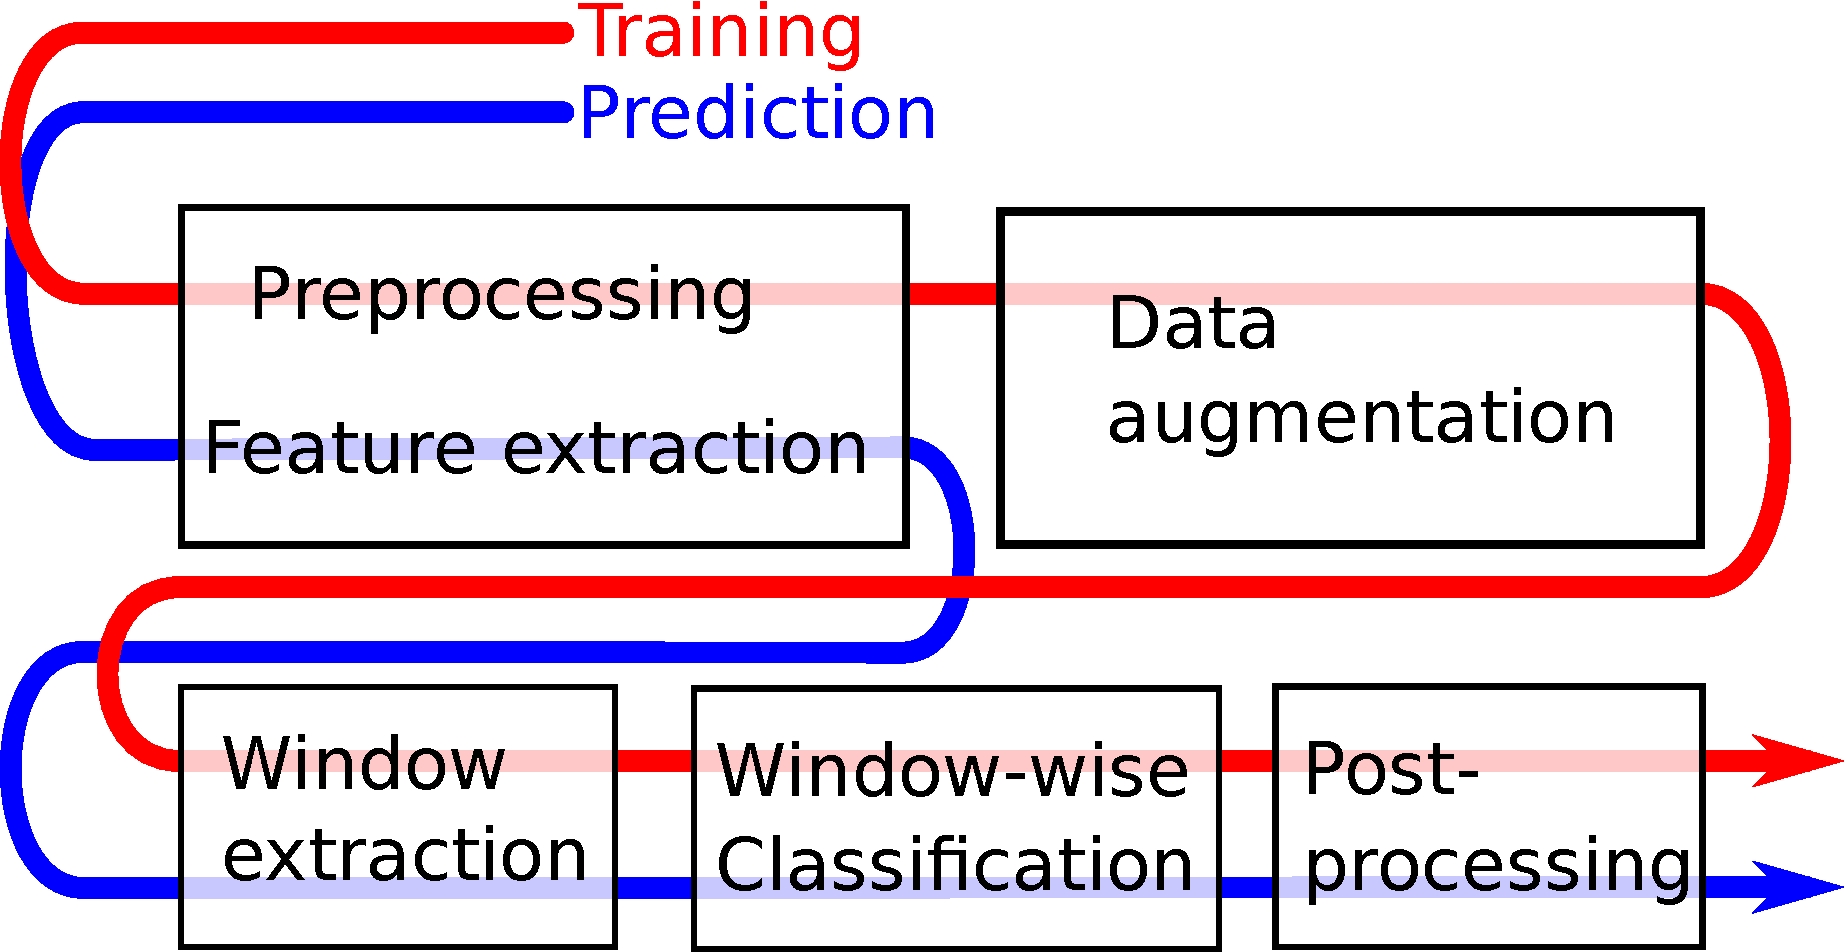
\includegraphics[width=\linewidth, keepaspectratio]{figures/segmentation-pipeline.pdf}
    \caption{A typical segmentation pipeline gets raw pixel data, applies
             preprocessing techniques like scaling and feature extraction like
             HOG features. For training, data augmentation techniques such as
             image rotation can get applied. For every single image, patches
             of the image called \textit{windows} get extracted and those
             windows get classified. The resulting semantic segmentation can
             get refined by simple morphologic operations or by more complex
             approaches such as \glspl{MRF}.}
    \label{fig:segmentation-pipeline}
\end{figure}

% TODO Figure: - Raw Pixel data Preprocessing / Feature extraction
% TODO ...:      ... this includes pyramids
% TODO ...:-> data augmentation to get more training material and invariance
% TODO ...:-> sliding window and a standard classifier
% TODO ...:-> post-processing to assure consistency

This approach was taken by~\cite{bittel2015pixel} and a majority of the VOC2007
participants~\cite{pascal-voc-2007}. As this approach has to apply the patch
classifier $512 \cdot 512 = \num{262144}$ times for images of size
$\SI{512}{\pixel} \times \SI{512}{\pixel}$, there are techniques for speeding
it up such as applying a stride and interpolating the results.

However, there are alternatives. Namely \glspl{MRF} and \glspl{CRF}
which take the information of the complete image and segment it in an holistic
approach.
